\documentclass[oneside, twocolumn, a4paper, 10pt]{IEEEtran}
\usepackage{caption}
\usepackage{url}
\usepackage[dvipsnames]{xcolor}
\usepackage{graphicx}
\usepackage{hyperref}
\usepackage{pdfpages}
\begin{document}
\title{Interpretable Clustering and Classification of an Imbalanced Dataset of DNA Sequences}
\author{Shekh Ahammed Adnan Bashir \\ Department of Computer Science and Engineering \\ Bangladesh University of Engineering and Technology \\ \url{1018052026@grad.cse.buet.ac.bd}}
\date{\today}
\maketitle

\begin{abstract}
Clustering or classification of DNA sequences is more difficult than doing those with any other type of sequence due to various reasons. Such tasks become more difficult when they have to be done on the genus or family. A further difficulty is added when the class samples vary in number- that is, the dataset of DNA sequences is imbalanced. However, through using proper feature extraction techniques and dataset sampling technique such tasks become feasible. The dataset we work in this paper has $9$ classes and the number of samples varies from $4$ to $1269$. In this work, we present a feature extraction technique inspired by popular Natural Language Preprocessing algorithm GloVe \cite{1} to make the classification and clustering of such a huge and imbalanced dataset possible. The feature extraction routine is static rather than being a learning one. This eased the interpretation of the machine learning tasks easier. Using interpretable shallow learning techniques, we achieved an accuracy score of around $99.8$\% and a V-measure of $0.5363$.
\end{abstract}

\section{Introduction}
With the rapid development of next-generation genome sequencing techniques, newer species are being classified quickly. It is important to know the class (family or genus) that a newly sequenced DNA belong to besides learning how the new species are related to the other ones. Here comes the necessity of DNA sequence classification and clustering. In both classification and clustering, a given collection of items is separated into a few to several subcollections so that the items in one subcollection are as similar as possible with items in two different subcollections are as different as possible. However, they differ in the way they do it.\\
\par
In classification, labeled data is provided to the classifier and the classifier learns an implicit measure of similarity upon seeing the labels of the provided data. This implicitly learned similarity measure can take a very complicated mathematical form. On the other hand, in clustering, a measure of similarity is provided explicitly and the clusterer separates the items into subcollections according to that similarity score. The clusterer does not need data labels. The better the similarity measure provided to the clusterer, the better the separation is and hence better the V-measure score is. As the similarity measure used in clustering is already understood, we can gain an insight into the data in the light of that. Broadly speaking, classification discovers the separating boundary in a given collection to divide that into subcollections and clustering is discovering the groups based on a provided similarity measure. Clustering provides us a view of how the items in a collection form homogeneous groups of items and classification draws decision boundaries among the groups.\\
\par 
A sequence is a list of elements. In a sequence, items of the provided collection are arranged one after another. There might or might not be sequential dependencies among the items. That is, the value of an item appearing in the latter positions might or might not depend on the value of items or items appearing in the previous positions. This dependency relation varies from problem to problem and this can only either be inferred from the data or provided to the algorithm as parameters. Classification and clustering tasks on the sequences hence are very difficult with data analysis and static algorithms only.\\
\par
DNA sequences are composed of $4$ different nucleotides- Adenine, Cytosine, Guanine, and Thiamine. Therefore, it is very likely that the DNA sequence of two species shares some common region because of the small state space. There are noises in the DNA sequences. There is an intra-class difference of the DNA sequences when it comes to classifying genus or families of DNA sequences. Through using preprocessing techniques that maintain the class invariant properties yet transforming all the sequences into sequences of the same length or extracting features we can successfully classify or cluster the sequences in such cases.\\
\par
Interpretability is important to better understand the data so that some static algorithms can be employed to do something of importance with a certain guarantee. When a classifier or a clusterer do their respective tasks, it can do so interpretable or not. Using static feature preprocessing and understanding the parameters and attributes of the machine learning models helps result interpretation. Decision tree-based classifiers, probabilistic classifiers, manifold learning algorithms provide interpretable results because there is a predefined step by step manner rather optimizing the decision boundary based on different hyperparameters only like black-box machine learning models.\\
\par
In this work, our main focus has been on interpreting the results obtained from the clusterer and the classifier. Specifically, our contributions are:
\begin{itemize}
\item Designing a feature extraction procedure that maintains the class invariant property of the DNA sequences.
\item Using interpretable machine learning techniques to cluster and classify the DNA sequences.
\item Interpretation of the results obtained from the clusterer and the classifier.
\end{itemize}

%
\section{Previous Works}
Better the features better the classification accuracy is. Works done so far on the classification of DNA sequences first extracts features. Nearly all the feature extraction procedure are hand engineered features. Also many of them do not employ popular classification algorithms on those hand-engineered extracted features. Many of them incorporates the use of very popular DNA sequence matching algorithm BLAST for thr discrimination of the sequences purpose. Wang et al. proposed two new methods to classify DNA sequences \cite{2}. The first technique relies on the comparison of a given sequence to a group of active motifs discovered from the classes it knows. The second technique generates and matches gapped fingerprints of a given unlabeled sequence with the elements of classes it knows. Stranneheim et al. classified DNA sequences through using Bloom filters to keep track of novelties of the sequence reads \cite{3}. Seo transformed sequence data to real-valued vectors so that Support Vector Machine (SVM) can be applied \cite{4} to the data for the purpose of classification. In MEGAN \cite{5}, a sequence is searched against multiple sequence databases for assigning the lowest common ancestor of the best matches in different databases to the sequence. PhymmBL \cite{6}, \cite{7} uses interpolated Markov models to characterize variable-length oligonucleotides and combines with BLAST matching score to yield better accuracy. The Na\"{i}ve Bayes classifier \cite{8} learns a Bayesian rule from the k-mer distribution of genomes in the training data and applies that rule to classify. In Kraken \cite{9}, each k-mer in the sequence is mapped to the lowest common ancestor (LCA) of the genomes that contain that k-mer in a database. For classifcation, the taxa associated with the k-mers in the sequence form a pruned subtree of the general taxonomy tree. Another classifier CLARK \cite{10} defines k-spectrum. k-spectrum of a string $x$ is the vector of dimension $4^k$ that collects the number of occurences of all possible k-mers in $x$. k-spectrum represents each DNA sequence. The CLARK algorithm first computes the k-spectrum of a unlabeled DNA sequence. Then the algorithm removes the common regions of the sequences to make the remaining k-mers to be discriminative. Finally, based on the maximum similarity in k-mer frequencies a class is assigned to an unlabeled DNA sequence.\\
\par
As we already discussed, clustering of DNA sequences is done to study the similarities among the DNA sequences through the lens of a predefined similarity measure. Plenty of works, such as DNACLUST \cite{11}, d2 cluster \cite{12}, CD-HIT \cite{13}, UCLUST \cite{14} have already been done to cluster DNA sequences and they are interpretable. However, seldom of them used adhoc clustering algorithms rather than the ones which are widely known and their inner workings are understood in depth. MeShClust \cite{15} addressed the issue of the sensitivity of clusterer output due to predefined algorithm paramaters. It repurposes the popular Mean Shift algorithm \cite{16} for the DNA sequence clustering. It is a nonparametric feature space analysis technique and seeks the maxima of a density function. The space spanned by DNA sequences can be considered as feature space. The distribution has a density function in that space and modes are the cluster in the input space. However, considering the maxima of the density function as in Mean Shift algorithm makes it very difficult to work with highly imbalanced training dataset- that is, if the number of samples from different classes varies largely.
\section{Dataset Description}
The dataset is a synthetic one. This dataset has been generated from the dataset for Microsoft Malware Classification challenge hosted on Kaggle \cite{21}. It is a plain encoding of the binary file using nucleotides A, C, G, T. The dataset is an imbalanaced one with the number of samples per class varying from $4$ to $1269$. The number of samples per class is tabled in \autoref{tab:classdescription}. 
\begin{table}
\begin{center}
\begin{tabular}{|c|c|}
\hline
Class & Number of samples\\ \hline
1 & $607$\\ \hline
2 & $852$\\ \hline
3 & $1269$\\ \hline
4 & $66$\\ \hline
5 & $4$\\ \hline
6 & $510$\\ \hline
7 & $4$\\ \hline
8 & $138$\\ \hline
9 & $356$\\ \hline
\end{tabular}
\caption{Class description of the dataset.}
\label{tab:classdescription}
\end{center}
\end{table}
Now we oversample the classes in the dataset randomly so that each class has equal number of samples. We did not subsample any class to be as inclusive of patterns as possible so that the classification accuracy remains high.
\section{Methodology}
\subsection{Sequence Embedding}
\subsubsection{Popular techniques}
Embedding is the process of mapping some signal from one domain to another. Embedding is done in order to obtain the data in a suitable format so that the machine learning algorithm can do its task conveniently. Sequence embedding maps an entire sequence to another domain. Sequence embedding eases the modeling the sequence for further tasks. Sequence modeling is predicting the distribution of the smaller units of the sequence. It also can be used to extract features of the sequences.\\
\par 
Feature extraction falls under the umbrella of feature learning. Feature extraction is done through discovering the patterns among the smaller units in the sequence. Feature extraction routines can be learning procedures or static procedures. Therefore, feature extraction can be done using static algorithms those rely on domain specific knowledge or hypotheses regarding the sequence or can be done using neural networks or shallow learning algorithms. Feature extraction can be done on both the raw data or on the embedded data. During embedding feature extraction is done implicitly. In our case the raw data are the sequences of A, C, T, and G and the embedded data are the embedding vectors for each of the sequences.\\ 
\par 
In the field of Natural Language Processing, word embedding, which is a sequence embedding technique, refers to a set of techniques for language modeling and feature learning. In NLP, word embedding is done on words or phrases to map them to real valued vectors. This real-valued vectors are used for further tasks- such as classification or clustering. There are severalp opular word embedding techniques including word2vec \cite{17}, GloVe \cite{18}, fastText \cite{19} \cite{20}, etc. Each of the routines transforms word sequences such as sentences, paragraphs, etc. into real valued vectors for feasible classification, clustering, etc.\\
\par 
word2vec reduces the number of dimensions using neural networks to learn the embedding. It produces the sequence embedding in two exclusive methods. In one method, called continuous bag of words, the feature learning model is trained to predict a word from the context or surrounding words of it. In another method, called skip-gram, the context words are predicted from a given word through assigning some probability score to a one hot vector of the vocabulary under consideration. GloVe uses a static method to produce the embedding. GloVe model is trained on aggregated global word-word co-occurrence statistics from a corpus. Representations obtained from GloVe demonstrate interesting linear substructures of the word vector space. fastText learns a representation for each character n-gram (a number of neighboring characters around a character in a word) instead of directly learning a vector representation for a word (as with word2vec). Each word is represented as a bag of character n-grams, so the overall word embedding is a sum of these character n-grams.
\subsubsection{Our approach}
We extend two sequence embedding techniques to the domain of biological sequences- word2vec and GloVe. However, rather directly using them, we modify them for using with k-mers. While using word2vec for generating an embedding, we used a neural network as an autoencoder. However, we could not have the training procedure converged. Later we went for a variant of the GloVe algorithm where we picked only the static part of generating the histogram. It worked fine. The intuition behind our embedding routine is that the probability of the presence of a particular $k$-mer in a predefined distance from a given $k$-mer varies among the genus. That is, within a specific genus, the this probability is almost the same.\\
\par
We first split the sequence into nonoverlapping subsequence of length $k$. We experimented with different values of $k$ and finally found that $k = 3$ works the best in our case. As k-mers we pick 3-mers, that is the codons. We did not pick the value of $k$ experimentally. We picked a value of $k$ that corresponds to a already known and studied biological structure. Then we construct a \textit{weighted} cooccurence vector out of that. To construct the vector we first define a number of neighbors on the right and the left side of a given k-mer and initialize a matrix of $0$s of dimension $4^k \times 4^k$. Here $4$ is the number of DNA bases and $k$ is the $k$ value of the k-mer we consider. Therefore, the rows and the columns of the matrix corresponds all possible k-mers. That is, an item $C_{i,j}$ is the weight of association between k-mer $i$ and k-mer $j$ in a given sequence. We call this matrix cooccurence matrix.\\
\par
We take maximum that number of left and right neighbor. For example, for a sequence of length $100 * k$ (k-mer sequence of length $100$) and left and right neighbor count of $3$, the first k-mer in the sequence we only have the right neighbor (k-mers in the $2^{nd}$, $3^{rd}$, and $4^{th}$ positions), the last k-mer has only left neighbors (k-mers in the $97^{th}$, $98^{th}$, and $99^{th}$ positions), and the $10^{th}$ k-mer has k-mers in $7^{th}$, $8^{th}$, and $9^{th}$ position as the left neighbors and k-mers in the $11^{th}$, $12^{th}$, and $13^{th}$ positions in the sequence as the right neighbors. Now we add $\frac{1}{3}$ to the weight between the k-mer at the $10^{th}$ position and the k-mer at the $7^{th}$ position and the k-mer at the $10^{th}$ position and the k-mer at the $13^{th}$ position. That is, we do $\mathbf{C}_{10, 7} = \mathbf{C}_{10, 7} + \frac{1}{3}$ and $\mathbf{C}_{10, 13} = \mathbf{C}_{10, 13} + \frac{1}{3}$. We also do $\mathbf{C}_{10, 8} = \mathbf{C}_{10, 8} + \frac{2}{3}$ and $\mathbf{C}_{10, 12} = \mathbf{C}_{10, 12} + \frac{2}{3}$ and finally, $\mathbf{C}_{10, 9} = \mathbf{C}_{10, 9} + 1$ and $\mathbf{C}_{10, 11} = \mathbf{C}_{10, 11} + 1$. Finally, we flatten the matrix to obtain the cooccurence vector, that is, $\vec{C} = \mathbf{C}_{1,1}, \ldots, \mathbf{C}_{1, N}, \mathbf{C}_{2, 1}, \ldots, \mathbf{C}_{2, N}, \ldots, \mathbf{C}_{N-1, N},\mathbf{C}_{N, 1}, \ldots, \mathbf{C}_{N, N}$. Later, we divide the vector with the largest element in it in order to normalize it. This is how we get feature vector of constant size. The significance of this vector can be thoght of to express cooccurence intensity between the k-mers.
\subsection{Visualization through dimension reduction algorithms}
Many datasets can be represented as a matrix, such that each row represents a set of attributes (or features or dimensions). Attributes describe a particular instance of something. Larger the number of attributes (columns) exponentially large the space of unique possible rows. Large number of data dimension causes difficulties in data sampling and pattern recognition. Reducing data into fewer dimensions often makes the analysis of algorithms more efficient, and can help machine learning algorithms make more accurate predictions.\\
\par
We want to have our clusters as nonoverlapping as possible. Visualization is important to understand how good our embedding routine is. We first visualize the clusters through dimension reduction algorithms. We pick three algorithms for that:
\begin{itemize}
\item Isomap
\item Locally-Linear Embedding (LLE)
\item T-distributed Stochastic Neighbor Embedding (t-SNE)
\end{itemize}
\begin{figure*}
\centering
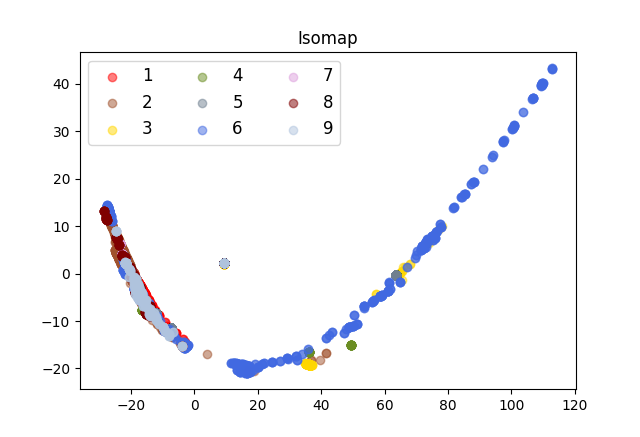
\includegraphics[width=0.6\linewidth]{../data/visualization/Isomap.png}
\caption{Isomap on the embeddings obtained from our embedding algorithm.}
\label{fig:isomap}
\end{figure*}
In Isomap first neighbors of each data point are found. Then a neighborhood graph is constructed with each point is connected to other if it is a $K$ nearest neighbor and edge length equal to Euclidean distance. Then in that neighborhood graph the shortest path between the nodes are computed. Finally, a lower-dimensional embedding is computed using multidimensional scaling. We notice that in the Isomap plot \autoref{fig:isomap} of our features many classes are largely overlapped.\\
\par
\begin{figure*}
\centering
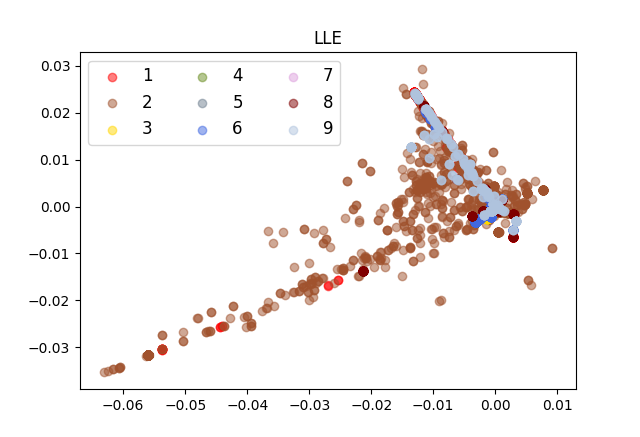
\includegraphics[width=0.6\linewidth]{../data/visualization/LLE.png}
\caption{Locally-Linear Enbedding on the embeddings obtained from our embedding algorithm.}
\label{fig:lle}
\end{figure*}
Locally-Linear Enbedding leverages the sparsity of the data matrix. First, LLE finds a set of the nearest neighbors of each point. Then it computes a set of weights for each point that best describes the point as a linear combination of its neighbors. Finally, an eigenvector-based optimization is done to find the low-dimensional embedding of points, such that each point is still described with the same linear combination of its neighbors. LLE does not have a mechanism to work with data points with nonuniform density. It performs poor in those cases. This is observed in our LLE plot \autoref{fig:lle}.\\
\par
\begin{figure*}
\centering
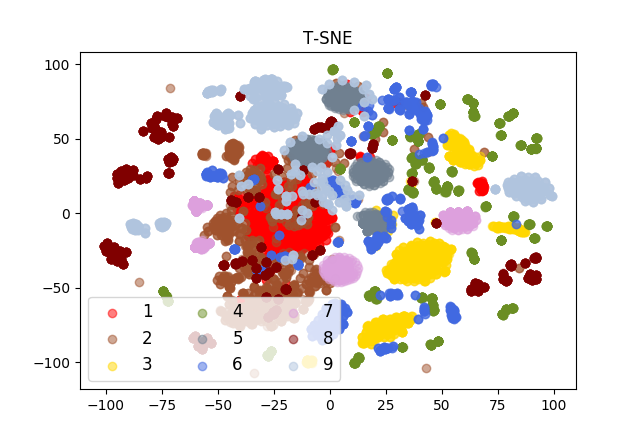
\includegraphics[width=0.6\linewidth]{../data/visualization/T-SNE.png}
\caption{T-distributed Stochastic Neighbor Embedding on the embeddings obtained from our embedding algorithm.}
\label{fig:tsne}
\end{figure*}
t-SNE models each high-dimensional data point by a two- or three-dimensional point in such a way that similar objects are modeled by nearby points and dissimilar objects are modeled by distant points with high probability. First, a probability distribution over pairs of high-dimensional objects is constructed. Second, a similar probability distribution is defined over the points in the low-dimensional map, and then t-SNE minimizes the Kullback–Leibler divergence between the two distributions with respect to the locations of the points in the map. Reducing dimensionality with t-SNE we are able to see the clusters better upon plotting \autoref{fig:tsne}. However, feeding this reduced dimensioned data to the classifiers does not yield better classification.\\
\par
This is error is due to the unsupervised nature of the dimension reduction algorithms. The classification boundary in all problems cannot be properly defined by the well-studied similarity measure(s) alone. Therefore, dimension reduction in an unsupervised fashion does not always work. This is the reason we did not reduce the data dimension for supervised training.
\subsection{Sequence Clustering}
There are broadly two types of sequence clustering algorithm on the basis of number of clusters as input parameter to the algorithm. Algorithms that do not require the number of clusters as an input parameter discover the clusters from the input data through using density functions or similar mathematical constructs.\\
\par
Clustering algorithms such as DNACLUST \cite{11}, d2 cluster \cite{12}, CD-HIT \cite{13}, UCLUST \cite{14} requires defining the number of clusters. However, this is difficult to guess the number of clusters beforehand in case of unlabled data. Although our dataset is labeled, we look into methods that do not require defining this number. One such tool is MeShClust \cite{15}. However, this tool is based on Mean Shift algorithm which relies on blob discovery and hence do not look into large overlapping clusters. We resort to Affinity Propagation \cite{22} which relies on \textit{message passing} among the data points to discover class representatives.\\
\par 
Affinity Propagation is an iterative algorithm. The algorithm proceeds by alternating two message passing steps, to update two matrices- the \textit{responsibility} matrix $\mathbf{R}$ with items quantifying how well-suited samples are as representative element and the \textit{availability} matrix $\mathbf{A}$ items of which represent how \textit{appropriate} it would be for a sample under examination to pick another sample as its exemplar, taking into account the preference of other data points for picking the latter as a representative. Iteration is stopped once until either the cluster boundaries remain unchanged over some iterations, or after predefined number of iterations.\\
\par 
We used Affinity Propagation to cluster and obtained a V-measure score of $0.5636$. V-measure score depends on homogeneity and completeness score of the clustering. If each cluster has data-points belonging to the same class label then the clusters are perfectly homogeneous cluster. Homogeneity exdpresses the closeness of the clustering algorithm being perfect. If all data-points belonging to the same class are clustered into the same cluster then it is a perfectly complete clustering. V-measure is the harmonic mean of these two scores.
\subsection{Sequence Classification}
For the purpose of sequence classification we used a Random Forest classifier to obtain a test accuracy of $99.8$\%. Our train-test split was $4:1$. However, with a train-test split of $3:2$, $2:3$, $1:4$, $1:9$, and $1:19$ the test accuracy was $99.3$\%, $98.8$\%, $96.9$\%, $93$\%, and $87.9$\% respectively. This evidences that in the embedding space embedded DNA sequences from each of the genus are well separated. This is also evidenced in the visualizations above. Random Forest classifier makes use of decision trees. Random Forest is a popular algorithm in data mining. Random Forest is invariant to different feature transformations. Therefore, it is well suited for the feature spaces which underwent many transformations.\\
\par
During the training time the algorithm builds a predefined number of decision trees. When an input is provided to the Random Forest algorithm, each of the decision trees constructed in it during the training independently outputs results on that input. Finally, the consensus of those results are taken. This consensus is the output of the Random Forest classifier.\\
\par 
The decision-trees are grown very deep to capture very irregular patterns. Therefore, they have low bias, but very high variance that is overfit their training sets. To reduce the variance Random forests grow multiple deep decision trees with each trees trained on different random parts of the same training set. Although this improves the accuracy but it becomes more difficult to interpret the results.\\
\par 
We used $5$ decision trees in our Random Forest classifier. Our splitting ciriterion was gini impurity index. The max depth is not defined. The nodes are expanded until all leaves are pure. When looking for the best split we looked at $64$ features among the $4096$ features. Samples were bootstrapped during growing the decision trees. As we already balanced the samples per different classes we did not have to consider issues regarding imablanced data. 
\section{Interpretation} 
We plot the decision trees used in the Random Forest classifier to have an interpretation of the model we are using. However, we do not know where and how the training dataset were splitted and hence could not be studied properly. We are attaching the decision tree plots as an appendix to this report.\\
\par 
Despite the random position of the dataset splitting, we note from the decision trees that, most of the trees have their root the $3800$s index of the embedded vectors. Therefore, we can consider that there must be some important splitting criterion lies around those positions.
\section{Conclusion}
The embedding suitable for this dataset eases up the classification task. However, the random nature of the classification algorithm used prevents us from having an exact picture of what is happening in the classifier. This in turn blurs our view into how the genus are distinct from each other. Despite these, we can do further analysis tasks in the important subregions of the embedded space. One such area of interest is the regin spanning from index position $3802$ to $3899$, especially $3827$- which is the root of two among five decision trees in the random forest. Future direction of this work includes applying this technique to other DNA sequence classification datasets and extending the embedding routine to include methods from other popular NLP embedding algorithms to see why they excel or fail. More importantly to design an embedding routine that makes the classification possible using one single decision tree.
%\includepdf{../src/visualizations/estimator_0-rotated.pdf}
\begin{thebibliography}{6}
\bibitem{1} J. Pennington, R. Socher, and C. Manning \textit{Glove: Global Vectors for Word Representation}. EMNLP, 14, page 1532--1543. (2014)
\bibitem{2} Wang JT, Rozen S, Shapiro BA, Shasha D, Wang Z, Yin M. \textit{New Techniques for DNA sequence classification}. In J Comput Biol. 1999 Summer;6(2):209-18.
\bibitem{3} Henrik Stranneheim1, Max K\"{a}ller, Tobias Allander, Bj\"{o}rn Andersson, Lars Arvestad and Joakim Lundeberg. \textit{Classification of DNA sequences using Bloom filters}. Vol. 26 no. 13 2010, pages 1595–1600, doi:10.1093/bioinformatics/btq230.
\bibitem{4} Seo, TK. \textit{Classification of nucleotide sequences using support vector machines}. J Mol Evol. 2010 Oct;71(4):250-67. doi: 10.1007/s00239-010-9380-9.
\bibitem{5} Huson D, Auch A, Qi J, Schuster S: \textit{MEGAN analysis of metagenomic data}. Genome Res 2007, 17:377–386.
\bibitem{6} Brady A, Salzberg S. \textit{Phymm and PhymmBL: metagenomic phylogenetic classification with interpolated Markov models}. Nat Methods 2009, 6:673–676.
\bibitem{7} Brady A, Salzberg S. \textit{PhymmBL expanded: confidence scores, custom databases, parallelization and more}. Nat Methods 2011, 8:367.
\bibitem{8} Rosen G, Garbarine E, Caseiro D, Polikar R, Sokhansanj B. \textit{Metagenome fragment classification using N-mer frequency profiles}. Adv Bioinformatics 2008, 2008:1–12.
\bibitem{9} Wood, Derrick E and Salzberg, Steven L. \textit{Kraken: ultrafast metagenomic sequence classification using exact alignments}. Genome Biology 2014, 15:R46.
\bibitem{10} Rachid Ounit, Steve Wanamaker, Timothy J Close, Stefano Lonardi \textit{CLARK: fast and accurate classification of metagenomic and genomic sequences using discriminative k-mers}. BMC Genomics (2015) 16:236 DOI 10.1186/s12864-015-1419-2.
\bibitem{11} Ghodsi,M., Liu,B. and Pop,M. (2011) \textit{DNACLUST: accurate and efficient clustering of phylogenetic marker genes}. BMC Bioinformatics, 12, 271.
\bibitem{12} Burke,J., Davison,D. and Hide,W. (1999) \textit{d2 cluster: a validated method for clustering EST and full-length cDNA sequences}. Genome Res., 9, 1135–1142.
\bibitem{13} Li,W. and Godzik,A. (2006) \textit{Cd-hit: a fast program for clustering and comparing large sets of protein or nucleotide sequences}. Bioinformatics, 22, 1658.
\bibitem{14} Edgar,R.C. (2010) \textit{Search and clustering orders of magnitude faster than BLAST}. Bioinformatics, 26, 2460–2461.
\bibitem{15} James, Benjamin T., Luczak, Brian B., Girgis, Hani Z. \textit{MeShClust: an intelligent tool for clustering DNA sequences}. Nucleic Acids Research, 2018, Vol. 46, No. 14 doi: 10.1093/nar/gky315
\bibitem{16} Comaniciu, D. Meer, P. \textit{Mean shift: A robust approach toward feature space analysis}. IEEE Transactions on Pattern Analysis and Machine Intelligence (2002)
\bibitem{17} Mikolov, Tomas; Sutskever, Ilya; Chen, Kai; Corrado, Greg S.; Dean, Jeff (2013). \textit{Distributed representations of words and phrases and their compositionality}. Advances in Neural Information Processing Systems. arXiv:1310.4546.
\bibitem{18} Pennington, J., Socher, R. and Manning, C. D. \textit{Glove: Global Vectors for Word Representation}. EMNLP 2014.
\bibitem{19} Joulin, A., Grave, E., Bojanowski, P., Mikolov, T. \textit{Bag of Tricks for Efficient Text Classification} (cite arxiv:1607.01759)
\bibitem{20} Bojanowski, P., Grave, E., Joulin, A.,  Mikolov, T. (2017). \textit{Enriching Word Vectors with Subword Information}. Transactions of the Association for Computational Linguistics.
\bibitem{21} Microsoft Malware Classification Challenge (BIG 2015), \url{https://www.kaggle.com/c/malware-classification/}
\bibitem{22} Brendan J. Frey, Delbert Dueck. \textit{Clustering by passing messages between data points}. Science. 315 (5814): 972–976.
\end{thebibliography}
\end{document}
